\documentclass[11pt,a4paper]{article}
\usepackage{amsmath,amsthm,amsfonts,amssymb,amscd}
\usepackage{enumerate} 
\usepackage{physics}
\usepackage{enumerate}
\usepackage{fancyhdr}
\usepackage{hyperref}
\usepackage{graphicx}
\hypersetup{colorlinks,
    linkcolor=blue,
    citecolor=blue,      
    urlcolor=blue
}
\usepackage{xurl}

\oddsidemargin0.1cm 
\evensidemargin0.8cm
\textheight22.7cm 
\textwidth15cm \topmargin-0.5cm

\newtheorem{theorem}{Theorem}
\newtheorem{corollary}{Corollary}
\newtheorem{lemma}{Lemma}
\newtheorem{proposition}{Proposition}

\theoremstyle{definition}
\newtheorem{remark}{Remark}
\newtheorem{definition}{Definition}
\newtheorem{observation}{Observation}
\newtheorem{note}{Note}
\newtheorem{hope}{Hope}
\newtheorem{warning}{Warning}
\newtheorem{problem}{Problem}
\newtheorem{fear}{Fear}
\newtheorem{question}{Question}

\newcommand{\Z}{\mathbb{Z}}
\newcommand{\R}{\mathbb{R}}
\newcommand{\C}{\mathbb{C}}
\newcommand{\Q}{\mathbb{Q}}
\newcommand{\A}{\mathbb{A}}

\usepackage{listings}
\usepackage{xcolor}

\definecolor{codegreen}{rgb}{0,0.6,0}
\definecolor{codegray}{rgb}{0.5,0.5,0.5}
\definecolor{codepurple}{rgb}{0.58,0,0.82}
\definecolor{backcolour}{rgb}{0.95,0.95,0.92}

\lstdefinestyle{mystyle}{
    backgroundcolor=\color{backcolour},   
    commentstyle=\color{codegreen},
    keywordstyle=\color{magenta},
    numberstyle=\tiny\color{codegray},
    stringstyle=\color{codepurple},
    basicstyle=\ttfamily\footnotesize,
    breakatwhitespace=false,         
    breaklines=true,                 
    captionpos=b,                    
    keepspaces=true,                 
    numbers=left,                    
    numbersep=5pt,                  
    showspaces=false,                
    showstringspaces=false,
    showtabs=false,                  
    tabsize=2
}

\lstset{style=mystyle}

\newcommand{\MultiSet}{\mathrm{MultiSet}}
\newcommand{\len}{\mathrm{len}}
\newcommand{\din}{\texttt{d\_in}}
\newcommand{\dout}{\texttt{d\_out}}
\newcommand{\T}{\texttt{T} }
\newcommand{\Relation}{\texttt{Relation}}
\newcommand{\X}{\mathcal{X}}
\newcommand{\Y}{\mathcal{Y}}
\newcommand{\True}{\texttt{True}}
\newcommand{\False}{\texttt{False}}
\newcommand{\clamp}{\texttt{clamp}}
\newcommand{\function}{\texttt{function}}
\newcommand{\float}{\texttt{float }}
\newcommand{\questionc}[1]{\textcolor{red}{\textbf{Question:} #1}}

\newcommand{\silvia}[1]{{ {\color{blue}{(silvia)~#1}}}}
\newcommand{\grace}[1]{{ {\color{purple}{(grace)~#1}}}}
\newcommand{\connor}[1]{{ {\color{teal}{(connor)~#1}}}}
\newcommand{\mike}[1]{{ {\color{green}{(mike)~#1}}}}
\newcommand{\todo}{{\textcolor{red}{TODO }}}


\title{Privacy Proofs for OpenDP: Clamping}
\author{S\'ilvia Casacuberta}
\date{Summer 2021}

\begin{document}

\maketitle

\tableofcontents

\section{Algorithm Implementation}
% OLD VERSION: The current OpenDP library contains two functions related to Clamping: \texttt{make\_clamp\_vec} and \texttt{make\_clamp\_sensitivity}. Both functions are contained in the file \texttt{manipulation.rs}. In this document, we are referring to the Clamping function \texttt{make\_clamp\_vec}.

% OLD VERSION: The current OpenDP library contains the \texttt{make\_clamp\_vec} function implementing the clamping function. This is defined in lines 68-80 of the file \texttt{clamp.rs} (\url{https://github.com/opendp/opendp/blob/21-impute/rust/opendp/src/trans/clamp.rs}).

\subsection{Code in Rust}
The current OpenDP library contains the \texttt{make\_clamp\_vec} function implementing the clamping function. This is defined in lines 25-38 of the file \texttt{manipulation.rs} in the Git repository\footnote{As of June 16, 2021. Since then, the code has been updated to include a more general clampable domain, which is not yet finished.} (\url{https://github.com/opendp/opendp/blob/58feb788ec78ce739caaf3cad8471c79fd5e7132/rust/opendp/src/trans/manipulation.rs#L25-L38}).

\begin{figure}[ht]
    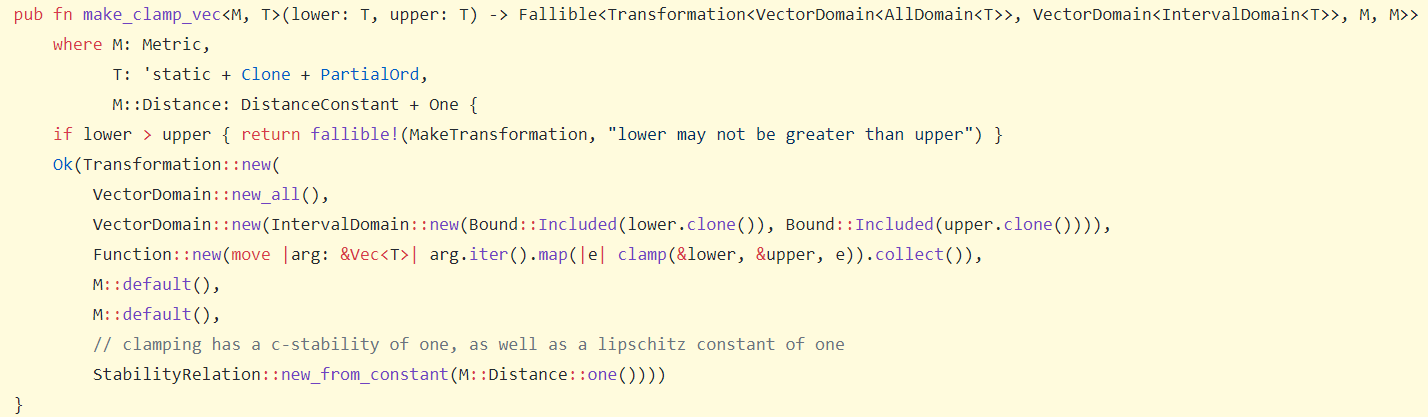
\includegraphics[width=16cm]{clamp_rust.png}
    \centering
    \label{fig:code}
\end{figure}

% Change: go back to the previous Git push.
% TODO: add clamp sensitivity?

\subsection{Pseudocode in Python}\label{sec:pseudocode}
We present a simplified Python-like pseudocode of the Rust implementation below. The necessary definitions for the pseudocode can be found at \href{https://www.overleaf.com/project/60d215bf90b337ac02200a99}{``List of definitions used in the pseudocode"}. 

%\silvia{We could generalize the input domain below from float to a any general (unspecified) type that admits total ordering, and then add the corresponding precondition to assert that the type \texttt{T} for $L$ and $U$ has the trait \texttt{TotalOrd}. Note that partial ordering is not enough, and we might not be able to clamp in the domain. However, TotalOrd is still not implemented in the OpenDP library.}

%\newpage

\subsubsection*{Preconditions}
To ensure the correctness of the output, we require the following preconditions:

\begin{itemize}
    \item \textbf{User-specified types:}
    \begin{itemize}
        \item Type \texttt{T} must have trait \texttt{TotalOrd}.\footnote{For now, the OpenDP library only implements \texttt{PartialOrd}, but \texttt{TotalOrd} will soon be implemented.}
    \end{itemize}
    \item \texttt{input\_domain:} any vector of elements of type \texttt{T}.
    \item \texttt{output\_domain:} any vector of elements of type \texttt{T} which are contained in the interval \texttt{[L, U]}, where 
    \texttt{L} and \texttt{U} are of type \texttt{T}. \silvia{Problem: \texttt{L} and \texttt{U} appear only later in the pseudocode, as discussed on July 13.}
    \item \texttt{input\_metric:} symmetric distance.
    \item \texttt{output\_metric:} symmetric distance.
\end{itemize}

\subsubsection*{Postconditions}
\begin{itemize}
    \item A \texttt{Transformation} is returned (i.e., if a \texttt{Transformation} cannot be returned successfully, then an error should be returned).
\end{itemize}

% Perhaps: change L for lower and U for upper
\begin{lstlisting}[language=Python, escapechar=|] 
def MakeClamp(L: T, U: T): |\label{line:def}|
    if L > U: raise Exception('Invalid parameters') |\label{line:excep}|
    def Relation(d_in: u32, d_out: u32) -> bool: |\label{line:rel}|
        return d_out >= d_in*1
    
    def function(data: Vec(T)) -> Vec(T): |\label{line:fn}|
        def clamp(x: T) -> T: |\label{line:clamp}|
            return max(min(x, U), L)
        return list(map(clamp, data)) |\label{line:map}|
    
    return Transformation(input_domain, output_domain, function, input_metric, output_metric, stability_relation)
\end{lstlisting}

% Mike said: go back to float (so the GitHub version before the merge). Also: the end user chooses the metric. But the library will only allow 6 possible metrics (maybe expanded in the future): symmetric, hamming, $\ell_1$, $\ell_2$, max divergence, and smooth max divergence. So, in the case of clamping, the input metric can only be either symmetric or hamming. I should have a proof for each.

% Flipping $\din, \dout$: The worst case is equality. The relation accepts all greater distances. That's why the inequality is reversed. After chaining, the end-user can run a search (e.g., binary search) to tighten the $\dout$ down to the inequality.

\smallskip

%\silvia{If input metric equals output metric, do as above to avoid having to check that the end user passed them equal and raise exceptions?}

%\silvia{Stability relation and defining $\din, \dout$.}

%\silvia{Assuming it is ok to say bounded\_float?}

% Mike: "You can use the total ordering construction-time check to justify that min and max in your function work with the argument and won't fail"

% Also important: Programming framework setting $\mathcal{X} = \mathbb{R}$ is equivalent to $AllDomain<T>$ where $T$: Float.

\section{Proof}
The necessary definitions for the proof can be found at \href{https://www.overleaf.com/project/60d214e390b337703d200982}{``List of definitions used in the proofs"}.

\subsection{Symmetric Distance}
%\todo{Assumptions on min and max functions? Only min is defined in Rust, and assumes PartialOrd.}

%\todo{The carry type in Rust; e.g., bounded R is f32. But since it is bounded, it must be between L and U, but this does not follow from f32.} 

%\todo{Change theorem statement to include all needed  so that the theorems are claims about the constructors}

%\silvia{Reference specific lines in the pseudocode? E.g., for function.}
\begin{theorem}
    For every setting of the input parameters \texttt{(L, U)} to \texttt{MakeClamp} such that the given preconditions
    hold, the transformation returned by \texttt{MakeClamp} has the following properties:
    \begin{enumerate}
        \item \textup{(Appropriate output domain).} For every element $v$ in \texttt{input\_domain}, $\function(v)$ is in \texttt{output\_domain}. % Prof. Vadhan said on 29/6 to leave it as this for now, but maybe in the future we add to the theorem statement what exactly the input domain and output domain are (although of course we already say this in the proof)
        
        \item \textup{(Domain-metric compatibility).} The domain \texttt{input\_domain} matches one of the possible domains listed in the definition of \texttt{input\_metric}, and likewise \texttt{output\_domain} matches one of the possible domains listed in the definition of \texttt{output\_metric}.
        
        \item \textup{(Stability guarantee).} For every pair of elements $v, w$ in \texttt{input\_domain} and for every pair $(\din, \dout)$, where $\din$ and $\dout$ are of type \texttt{u32}, if $v,w$ are $d_{in}$-close under \texttt{input\_metric} and $\Relation(\din, \dout) = \True$, then $\function(v), \function(w)$ are $d_{out}$-close under \texttt{output\_metric}.
    \end{enumerate}
\end{theorem}

\begin{proof}
\textbf{(Appropriate output domain).} In the case of \texttt{MakeClamp}, this corresponds to showing that for every vector $v$ of elements of type \texttt{T}, $\function(v)$ is a vector of elements of type \texttt{T} which are contained in the interval \texttt{[L, U]}. For that, we need to show two things: first, that \texttt{function(v)} has type \texttt{Vec(T)}. % Recall that the compiler infers the float type from VectorDomain(IntervalDomain(L, U)) because L and U have type float
Second, that they belong to the interval \texttt{[L, U]}.

Firstly, that $\function(v)$ has type \texttt{Vec(T)} follows from the assumption that element $v$ is in \texttt{input\_domain} and from the type signature of \texttt{function} in line~\ref{line:fn} of the pseudocode (Section~\ref{sec:pseudocode}), which takes in an element of type \texttt{Vec(T)} and returns an element of type \texttt{Vec(T)}. If the Rust code compiles correctly, then the type correctness follows from the definition of the type signature enforced by Rust. Otherwise, the code raises an exception for incorrect input type. 

Secondly, we need to show that the vector entries belong to the interval \texttt{[L, U]}. This follows from the definition of \texttt{clamp} in line \ref{line:clamp}. According to line \ref{line:clamp} in the pseudocode, there are 3 possible cases to consider:
\begin{enumerate}
    \item \texttt{x} $>$ \texttt{U}: then $\clamp\texttt{(x)}$ returns \texttt{U}.
    \item \texttt{x} $\in$ \texttt{[L, U]}: then $\clamp\texttt{(x)}$ returns \texttt{x}.
    \item \texttt{x} $<$ \texttt{L}: then $\clamp\texttt{(x)}$ returns \texttt{L}.
\end{enumerate}
In all three cases, the returned value of type \T is contained in the interval \texttt{[L, U]}. Hence, the vector $\function(v)$ returned in line~\ref{line:map} of the pseudocode is an element of \texttt{output\_domain}.

Lastly, the necessary condition that \texttt{L} $\leq$ \texttt{U} is checked in line~\ref{line:excep} of the pseudocode, hence correctness is guaranteed if no exception is raised. Both \texttt{L} and \texttt{U} have type \texttt{T} by their precondition requirement. Both the definition of \texttt{IntervalDomain} and that of the \texttt{clamp} function (line~\ref{line:clamp} in the pseudocode, which uses the \texttt{min} and \texttt{max} functions) require that the type of \texttt{L, U}, and of each vector entry in $v$ implements \texttt{TotalOrd}. In the case of \texttt{T}, this holds by the preconditions.

%Next we show that the stability relation as defined in Equation~\eqref{eq:relation} yields a valid transformation. %\grace{Oh I think I understand now we assume $d_{in} \leq d_{out}$}

%\begin{lemma}[Soundness of the stability relation]\label{lemma:stability}
% Give it a name
%For every $(\din, \dout)$ pair, the function $\Relation(\din, \dout)$ returns $\False$ whenever there exists some $x$ such that $d_{\X}(x, x') \leq \din$ and $d_{\Y}(T(x), T(x')) > \dout$,
%where $T$ denotes the clamping transformation. %and $\Relation(\din, \dout)$ the clamping stability relation. % defined in pseudocode xx; specify where the Relation is defined better
%\end{lemma}

% Must show that the relation fails for every $(d_{in}, d_{out})$ pair where there exists some $x$ such that $d_{\mathcal{X}}(x, x') \leq d_{in}$ and $d_{\mathcal{Y}}(T(x), T(x')) > d_{out}$.

%\begin{proof}
%Since clamping is 1-stable, $d_{\Y}(T(x), T(x')) \leq d_{\X}(x, x')$ for all $x, x' \in \X$. (This is a recursive argument with Theorem 2! I think it has to go)
%\end{proof}
        
% MS EDIT1: I adjusted the statement to negate it-- the relation must fail for every pair that does not uphold the worst-case change in distances. It is fine for the relation to also fail for valid pairs-- there are many proofs out there that are not tight. Put another way, the relation need only fail everything that is not DP, it does not need to accept everything that is DP.

% Should "input parameters" be more specified?
% "appropriately quantified" sounds vague
%\grace{Why is this called privacy guarantee and not stability something? I thought it should only be a "privacy guarantee" for measurements not transformations.}
%\silvia{So ``privacy relation" for measurements $=$ ``stability relation" for transformations, but both are providing the DP guarantee. But maybe ``DP guarantee" is not the best name}

\smallskip
\textbf{(Domain-metric compatibility).}  For \texttt{MakeClamp}, both cases correspond to showing that \texttt{VectorDomain(T)} is compatible with symmetric distance. This follows directly from the definition of symmetric distance, as stated in \href{https://www.overleaf.com/project/60d214e390b337703d200982}{``List of definitions used in the proofs"}. The \textit{appropriate output domain property} shown above ensures that \texttt{output\_domain} is \texttt{VectorDomain(T)}, and hence also compatible with the \texttt{output\_metric} symmetric distance.

\smallskip
\textbf{(Stability guarantee).} Throughout the stability guarantee proof, we can assume that $\function(v)$ and $\function(w)$ are in the correct output domain, by the \textit{appropriate output domain property} shown above. 

Since by assumption $\Relation(\din, \dout) = \True$, by the \texttt{MakeClamp} stability relation (as defined in line~\ref{line:rel} in the pseudocode), we have that $\din \leq \dout$. Moreover, $v, w$ are assumed to be $\din$-close. By the definition of the symmetric difference metric, this is equivalent to stating that $d_{Sym}(v, w) = |\MultiSet(v) \Delta \MultiSet(w)| \leq \din$.

Further, applying the histogram notation,\footnote{See \textit{A Programming Framework for OpenDP}, footnote 1 in page 3. Note that there is a bijection between multisets and histograms, which is why the proof can be carried out with either notion. For further details, please consult \url{https://www.overleaf.com/project/60d214e390b337703d200982}.}  it follows that
\[
d_{Sym}(v, w) = \lVert h_{v} - h_{w}\rVert_1 = \sum_z |h_v(z) - h_w(z)| \leq \din \leq \dout.
\]
We now consider $\MultiSet(\function(v))$ and $\MultiSet(\function(w))$.
For each element $z \in \MultiSet(v) \cup \MultiSet(w)$, where $z$ has type \texttt{T}, if $z \in \MultiSet(v) \Delta \MultiSet(w)$, we will assume wlog that $z \in \MultiSet(v) \setminus \MultiSet(w)$. We consider the following cases:
%either $z \in \MultiSet(v) \cup \MultiSet(w)$ or $z \in \MultiSet(v) \Delta \MultiSet(w)$. In the former case, irregardless of whether $z \in [L, U]$ or $z>U, z<L$, element $z$ leaves $||h_v - h_w||_1$ invariant (by the definition of symmetric difference).

%In the latter case, assume wlog that $z \in \MultiSet(v)$ but $z \notin \MultiSet(w)$. We split the proof into three cases, and let $k$ be the multiplicity of $z$ in $\MultiSet(v)$.  
\begin{enumerate}
    \item $z >$ \texttt{U} or $z <$ \texttt{L}: then, in the former case, $\clamp(z) =$ \texttt{U}. First consider the case when $z \in \MultiSet(v) \cup \MultiSet(w)$ with the same multiplicity in both multisets. Then, $|h_{\function(v)}(z) - h_{\function(w)}(z)| = 0$ because we have both $h_{\function(v)}(z) = 0$ and $h_{\function(w)}(z) = 0$. Thus the sum
    \[
    \sum_z |h_{\function(v)}(z) - h_{\function(w)}(z)|
    \]
    remains invariant, because the quantity $|h_{v}(z) - h_{w}(z)|$ is added to $|h_{\function(v)}(\texttt{U}) - h_{\function(w)}(\texttt{U})|$, given that $\clamp(z) = \texttt{U}$. 
    
    %\grace{Good explanation, especially w word invariant.}
    
    Suppose $z$ has multiplicity $k_v \geq 0$ in $\MultiSet(v)$ and multiplicity $k_w \geq 0$ in $\MultiSet(w)$, where $k_v \neq k_w$. After considering $z$, the value $h_{\function(v)}(\texttt{U})$ becomes $h_{\function(v)}(\texttt{U}) + k_v$, and $h_{\function(w)}(\texttt{U})$ becomes $h_{\function(w)}(\texttt{U}) + k_w$. Hence the quantity $|h_{\function(v)}(\texttt{U}) - h_{\function(w)}(\texttt{U})|$ increases by at most $|h_v(z) - h_w(z)|$, since, by the triangle inequality,
    \[
         |(h_{\function(v)}(\texttt{U}) + k_v) - (h_{\function(w)}(\texttt{U}) + k_w)| \leq
    \]
    \[
         \leq |h_{\function(v)}(\texttt{U}) - h_{\function(w)}(\texttt{U})| + |k_v - k_w| =
    \]
    \[
        = |h_{\function(v)}(\texttt{U}) - h_{\function(w)}(\texttt{U})| + |h_v(z) - h_w(z)|.
    \]
    
    %It is only at most because if $h_{\clamp_{L, U}(v)}(U) < h_{\clamp_{L, U}(W)}(U)$ whenever $k_v > k_w$, or if $h_{\clamp_{L, U}(v)}(U) > h_{\clamp_{L, U}(W)}(U)$ whenever $k_v < k_w$
    %before considering this particular value of $z$, then after clamping $z > U$ their difference can shrink.
    
    %\[
     %   |h_{\clamp_{L, U}(v)}(U) - h_{\clamp_{L, U}(w)}(U)| = |h_v(U) - h_w(U)| + |h_{\clamp_{L, U}(v)}(z) - h_{\clamp_{L, U}(w)}(z)|.
    %\]
    
    The same argument applies whenever $z < \texttt{L}$. 
    
    \silvia{The first subcase discussed here, i.e., when $k_v = k_w$, is also proven by the triangle inequality expression above, but it seemed clean to separate the case where the total sum remains invariant.}
    %Therefore, we conclude that, in this case,
    %\[
     %   ||h_{\clamp_{L, U}(v)} - h_{\clamp_{L, U}(w)}||_1 - |h_v(z) - h_w(z)|
     %\leq |h_{\clamp_{L, U}(v)}(U) - h_{\clamp_{L, U}(v)}(U)|. 
    %\]
    
    \item $z \in \texttt{(L, U)}$: then, $\clamp(z) = z$. Since $h_v(z) = h_{\function(v)}(z)$ and $h_v(w) = h_{\function(w)}(z)$, it follows that $|h_v(z) - h_w(z)| = |h_{\function(v)}(z) - h_{\function(w)}(z)|$. Hence the histogram count, i.e., the quantity
     \[
        \sum_z |h_{\function(v)}(z) - h_{\function(w)}(z)|,
    \]
    remains invariant.
    
    % \item $z \leq L$: then, $\clamp_{L, U}(z) = L$. Then, $\clamp_{L, U (v)}(z) = \clamp_{L, U (w)}(z) = U$, and hence $|h_{\clamp_{L, U}(v)}(z) - h_{\clamp_{L, U}(w)}(z)| = 0$.
    
    \item $z = \texttt{U}$ or $z = \texttt{L}$: then, in the former case, $\clamp(z) = \texttt{U}$. If $z \in \MultiSet(v) \cup \MultiSet(w)$ with the same multiplicity in both multisets, then the histogram count remains invariant under the addition of element $z$. Otherwise, if $z \in \MultiSet(v) \setminus \MultiSet(w)$, or if $z$ is in their union but with different multiplicity, then element $z$ can increase the quantity $|h_{\function(v)}(\texttt{U}) - h_{\function(w)}(\texttt{U})|$ by at most $|h_v(z)-h_w(z)|$, following the same reasoning with the triangle inequality as in case~2.
    
    The same argument applies whenever $z = \texttt{L}$.
    % Probably simplify to add this case in the others.
\end{enumerate}

%\silvia{Make cases more concise; avoid repetitions (esp. to try to make proofs ``automatic")}

By aggregating the three cases above, we conclude that
\[
\sum_z |h_{\function(v)}(z) - h_{\function(w)}(z)| \leq \sum_z |h_v(z) - h_w(z)|.
\]
By the initial assumptions, we recall that $\din \leq \dout$, and that $v, w$ are $\din$-close. Then,
\[
\sum_z |h_{\function(v)}(z) - h_{\function(w)}(z)| \leq \sum_z |h_v(z) - h_w(z)| \leq \din \leq \dout.
\]
Therefore, 
\[
|\MultiSet(\function(v)) \Delta \MultiSet(\function(w))| \leq \dout,
\]
as we wanted to show.
\end{proof}

\silvia{Maybe add domain of $z$ below the sum?}
%\grace{Great, very rigorous}
% correct domains above?

% More proofs? Mike: Most proofs give conditions for which they are valid on. This mostly captures domains and metrics. You need a proof for the relation-- the function pseudocode, domains and metrics are all necessary to qualify the proof. I guess it may also make sense to have a proof for the output domain.

% Not sure: separate into vec and sensitivity?

\end{document}
